\chapter{Future Directions}\label{ch:future_directions}
\dsp

\section{Introduction}
In the last chapters, I discussed the environmental applications of GO. If a killer application of GO is to be found in the future, we might expect a significant ramp-up of production. In turn, this could lead to an increase in the amount of GO released into the environment, raising the concern of potential toxicological impacts and risks associated with GO exposure. Researchers should begin to assess GO toxicity in order to limit risks connected to human exposure. This line of research falls under recent EPA efforts to address the toxicity and the presence in the environment of contaminants of emerging concerns, including nanomaterials (NMs), which are also regulated by the Toxic Substances Control Act (TSCA). The EPA defines carbon NMs to be stable, have limited reactivity, composed entirely of carbon, and be strong antioxidants. GO cannot be included in this category due to its oxy-functionality and its metastability\cite{han2019simulating} and might  require an additional category.

\section{Graphene Oxide Toxicity}
There are two main mechanisms of GO-induced toxicity and cell damage (Fig.~\ref{Fig1_fut}). The first one relies on the physical interactions between the 2-D GO morphology and the cell membrane. In this mechanism, the sharp edges of GO can cut, penetrate, and disrupt the cell membrane. \cite{li2013graphene} The second mechanism is oxidative stress that can increase the generation of intracellular reactive oxygen species (ROS) and charge transfer. This process can cause lipid peroxidation and DNA damage, thereby disrupting cell membranes, inhibiting important metabolic functions of macromolecules, and leading to toxic effects in the cells.\cite{sanchez2011biological}

\begin{figure}[t!]
  \centering
  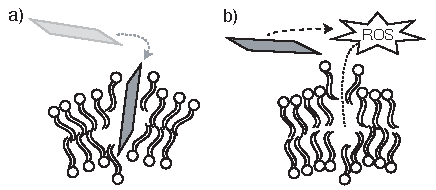
\includegraphics[width=5in]{future/Fig1.pdf}
  \caption{\textbf{GO nanotoxicity.} \textbf{(a)}  Direct physical damage to the cell membrane. \textbf{(b)} Indirect damage to the cell membrane via ROS and surface charges.}
  \label{Fig1_fut}
\end{figure}

Both mechanistic explanations (\textit{i.e.}, physical damage and oxidative stress) were reported 
to have bactericidal effects. For example, it has been proposed that a higher defect surface density in small GO flakes as compared to large flakes will induce oxidative stress and reduce bacterial adhesion. Other studies noted that damage of the model bacterium (\textit{E. coli}) by GO requires nanosheets penetration of the cell membrane, suggesting that a vertically aligned GO structure can lead to a greater antibacterial effect.\cite{lu2017enhanced} The importance of the structure and morphology was also corroborated by another finding showing that the bactericidal activity was dependent on  the morphology and the size of the GO flakes being similar to those of the bacteria.\cite{buccheri2016modification} The range of possible interactions depends on the environment and the medium in which GO is immersed, highlighting once again the importance of the presence of surface functionality.\cite{zhang2016mitigation}
The toxicity mechanisms might be largely distinct when applied to different cell lines in vitro, especially for eukaryotic cells that are more relevant to humans. Recently, carbon radicals were found to be the dominant surface functionality that induces cytotoxicity in lung cells.\cite{li2018surface} Other investigations reported that GO exposure can lead to lung cell apoptosis and granuloma formation only at high concentrations.\cite{chang2011vitro} The compatibility of GO with different oxidation states was studied in vivo, demonstrating that a reduced GO leads to rapid immune cell infiltration, uptake, and clearance from the injection site. \cite{sydlik2015vivo}\\
Since GO toxicity seems to be a function of GO purity, size, surface charge, functionalization and aggregation state, one could imagine mitigating GO toxicity by controlling its chemo-morphological properties.\cite{zhang2016mitigation}However, knowledge of GO fate and interaction in the human body is still limited and more investigations are needed to fully understand the mechanisms of toxicity.


\section{Proposed Experiments}
Human exposure to GO and nanomaterials, in general, can occur in several ways (\textit{e.g.}, ingestion, inhalation, injection, and dermal exposure) depending on the GO source and activities of the person. Since this thesis focuses on GO for water treatment applications, we identify ingestion as the main exposure mechanism.\\
As specified multiple times throughout this dissertation, GO is a metastable material, with a high potential for chemical interactions upon immersion in biological fluids. These interactions can induce phase transformation and dramatically modify GO chemo-morphological properties. In this sense, the relevant biological response and toxicity are not the ones of the original material, but rather, of its transformed configurations.  Transformations can also occur in the human body, which interacts with the nanomaterial and its intermediate states that arise during the transformation process.\cite{wang2016biological}\\
To study the gastrointestinal fate of GO, we proposed an experiment in which GO is passed through a three-stage gastrointestinal tract (GIT) simulator that includes the mouth, stomach, and small intestine (see Fig.~\ref{Fig2_fut}). The design assumes ingestion as the main exposure mechanism and is based on the GIT simulator developed earlier by \textit{Deloid et al.}. \cite{deloid2017integrated}

\begin{figure}[t!]
  \centering
  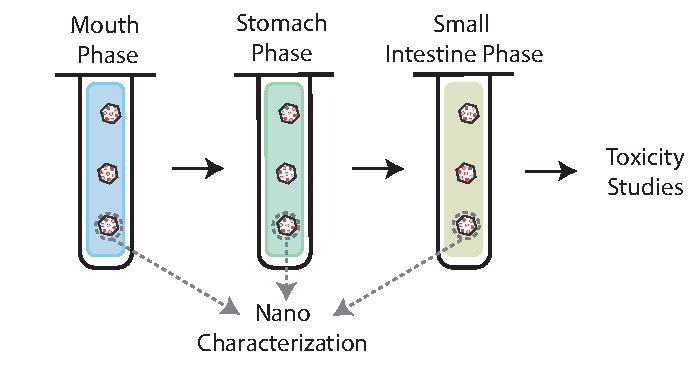
\includegraphics[width=5in]{future/Fig2.pdf}
  \caption{\textbf{Schematic of proposed experiments.} The experiments involve the GIT simulator, nanocharacterization and  toxicity studies.}
  \label{Fig2_fut}
\end{figure}


The initial GO concentration was 0.50 mg/mL. After digestion, the samples were diluted in serum-free DMEM cell culture medium so that the final concentration of the digested GO reached 10 $\mu$g/mL. One hundred (100) $\mu$L of the diluted digests was used to expose a near confluent cell monolayer. The GO concentration was calculated from the mass of  GO released if a GO-based membrane would break.
Nanotoxicity was evaluated by exposing digested GO to human cells and evaluating cell viability, using Invitrogen\textsuperscript{TM}'s PrestoBlue\textsuperscript{TM} cell viability assay. The resazurin dye in the Prestoblue\textsuperscript{TM} reagent is cell permeable. Once inside cells, it can be irreversibly reduced to the fluorescent resorufin. Since redox reactions are an indication of cell proliferation and cell viability, this dye can be used as an indicator of nanomaterial toxicity. Per manufacturer's guidelines, 24 hours after exposure, the diluted digests were carefully aspirated and the cells were washed with 100$\mu$L of PBS. Then, fresh Dulbecco's Modified Eagle Medium (DMEM) with 10\% PrestoBlue\textsuperscript{TM} reagent was added to the cells. The well plate was incubated at 37\textdegree C for 1 hour, and the fluorescence of the cells was measured at 560/590 nm (excitation/emission wavelengths). Any potential interference of GO with the assay were also measured. Cells were also exposed to a digest of phosphate buffer to measure the impact on viability due to the native composition of the digest. Ten (10) wells were allocated to each exposure condition. The statistical significance was set at $p = 0.05$ and was tested using an unpaired, parametric, two-tailed t-test.\\
Concurrently, the morphology and the chemistry of digested GO were characterized with surface science techniques in order to highlight possible transformations from the original (\textit{i.e.}, not digested) material. 

\section{Preliminary Results and Future Investigations}
The chemical transformation of the digested GO is displayed in the C1s XPS spectra (Fig.~\ref{Fig3_fut}a). The GO before digestion is characterized by O/C$\approx0.5$ with oxygen functionalities (epoxide, hydroxide, and carboxylate groups) previously observed throughout this thesis. On the other hand, we notice a strong reduction of the digested GO with a 50\% decrease in the O/C. The reduction process is also confirmed by the change in the oxygen functionality with an increase of the sp\textsuperscript{2} bonding (C-C and C=C) centered at 295 eV and a decrease of the single C-O bond (O-C-O and C-OH) centered at 297 eV. The reduction process could be connected to reducing agents present in the GIT. In particular, citrates and bases (NaOH) have been previously reported to reduce GO oxygen content. (reference deoxygenation, Facile synthesis of well dispersed ). We also notice the presence of $\approx3$\% nitrogen, which could be the residue of adsorbed proteins and urea acid used to simulate the GIT. Fig.~\ref{Fig3_fut}b shows the GO size distribution obtained by SEM before and after digestion and we did not observe a significant change in size.
\begin{figure}[h]
  \centering
  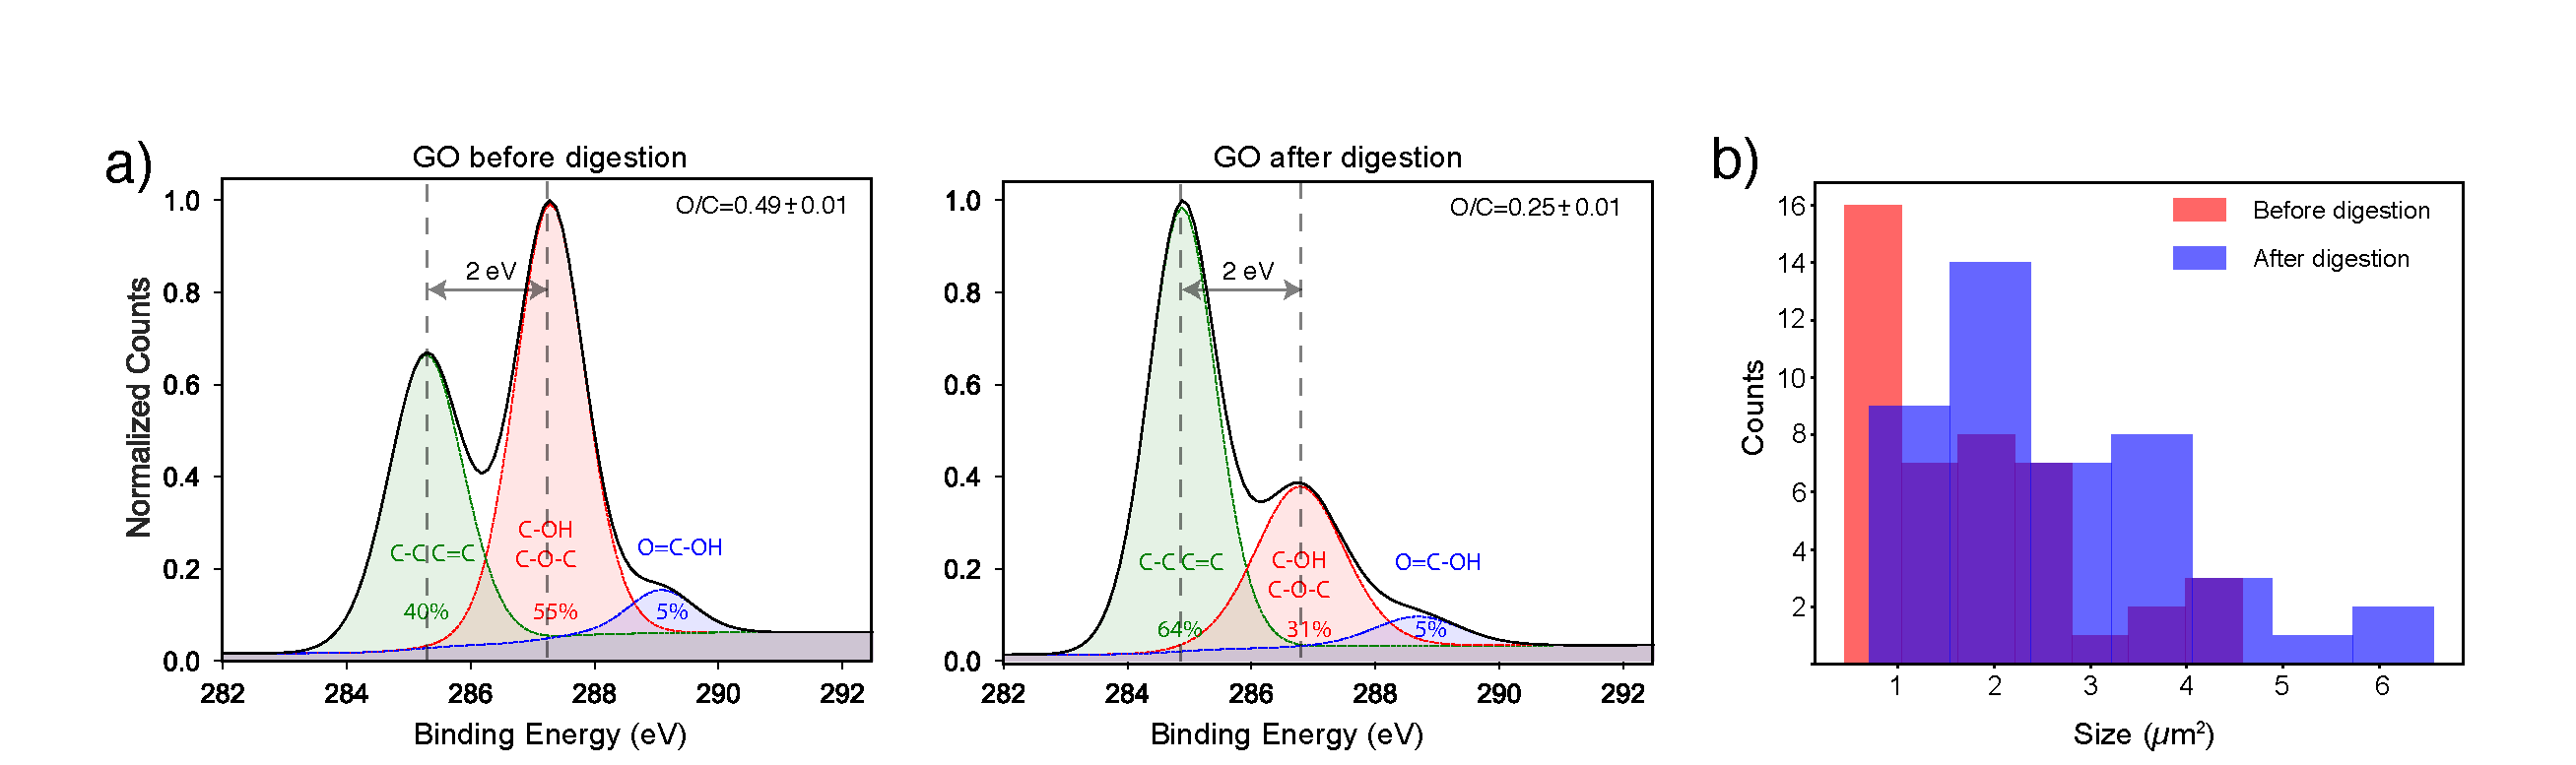
\includegraphics[width=6.5in]{future/Fig3.pdf}
  \caption{\textbf{Characterization of pristine and digested GO.} \textbf{(a)} XPS C1s spectra and \textbf size distribution analysis by SEM.}
  \label{Fig3_fut}
\end{figure}

Fig.~\ref{Fig4_fut} shows the viability of human epithelial colorectal adenocarcinoma (Caco-2) cells, previously seeded in 96-well plate. From Figure 4 we can observe that there is not a significant effect of the GO (digested or not) on cell toxicity. Cell viability is close to 100\% and similar to the control (CM or blank digest). Thus, GO at that concentration does not represent a meaningful biological concern.\\

These preliminary results form the foundation for a more robust study that will include: i) size distribution of the digested GO through laser diffraction in order to highlight possible agglomeration of the material in the GIT; ii) different combinations of GO chemistry and morphology in order to evaluate the effect of GO nanoproperties on toxicity; iii) conducting the nanotoxicity study on a co-culture model of the human gut epithelium (Caco-2 + HT29 cells) to more accurately mimic the intestinal environment.
\begin{figure}[t]
  \centering
  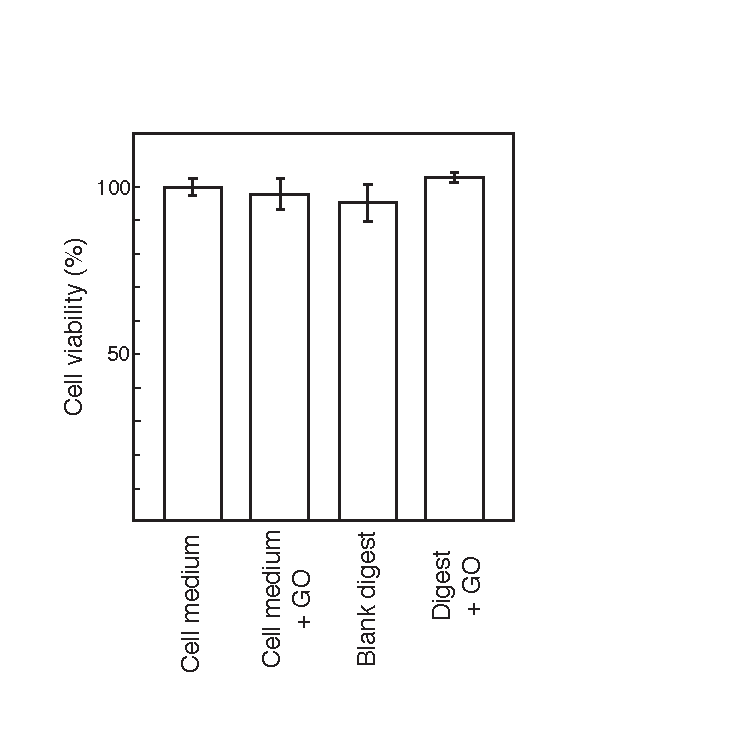
\includegraphics[width=5in]{future/Fig4.pdf}
  \caption{\textbf{Cell viability exposed to different media.}}
  \label{Fig4_fut}
\end{figure}

Further assays, including the production of ROS and cellular integrity, will also be considered.


